\documentclass[12pt, a4paper, oneside]{book}
\usepackage[hidelinks]{hyperref}
\usepackage[slovak]{babel}
\usepackage{epsfig}
\usepackage{epstopdf}
\usepackage[chapter]{algorithm}
\usepackage{algorithmic}
\usepackage{listings}
\usepackage{amsmath}
\usepackage{amssymb}
\usepackage{graphicx}
\usepackage{multirow}
\usepackage{color}
\usepackage{url}
\usepackage[utf8]{inputenc}
\usepackage[T1]{fontenc}
\usepackage{setspace}
\usepackage{tabularx}
\usepackage{textcomp}
\usepackage{caption}
\usepackage{natbib}
\usepackage{nopageno}


\setstretch{1.5}
%\renewcommand\baselinestretch{1.5} % riadkovanie jeden a pol

% pekne pokope definujeme potrebne udaje
\newcommand\mftitle{Algorithm development for the segmentation of astronomical images with unique features}
\newcommand\mfthesistype{Masters Thesis}
\newcommand\mfauthor{Bc. Viktor Nagy}
\newcommand\mfadvisor{prof. RNDr. Jiri Silha, PhD.}
\newcommand\mfplacedate{Bratislava, 2014}
\newcommand\mfuniversity{UNIVERZITA KOMENSKÉHO V BRATISLAVE}
\newcommand\mffaculty{FAKULTA MATEMATIKY, FYZIKY A INFORMATIKY}
\newcommand{\sub}[1]{$_{\text{#1}}$}
\newcommand{\reference}[1]{č.~\ref{#1}}
\newcommand{\imageHeight}{150px}

\ifx\pdfoutput\undefined\relax\else\pdfinfo{ /Title (mftitle) /Author (\mfauthor) /Creator (PDFLaTeX) } \fi

\begin{document}

\frontmatter

\thispagestyle{empty}

\noindent
\begin{minipage}{\textwidth}
\begin{center}
\textbf{\mfuniversity \\
\mffaculty}
\end{center}
\end{minipage}

\vfill
\begin{figure}[!hbt]
	\begin{center}
		
\includegraphics{images/logo_fmph}
		\label{img:logo}
	\end{center}
\end{figure}
\begin{center}
	\begin{minipage}{0.8\textwidth}
		\centerline{\textbf{\Large\MakeUppercase{Algorithm development for the segmentation}}}
		\centerline{\textbf{\Large\MakeUppercase{of astronomical images with unique features}}}
		\smallskip
		\centerline{\mfthesistype}
	\end{minipage}
\end{center}
\vfill
2014 \hfill
\mfauthor
\eject 
% koniec obalu

\thispagestyle{empty}

\noindent
\begin{minipage}{\textwidth}
\begin{center}
\textbf{\mfuniversity \\
\mffaculty}
\end{center}
\end{minipage}

\vfill
\begin{figure}[!hbt]
\begin{center}

\includegraphics{images/logo_fmph_dark}
\label{img:logo_dark}
\end{center}
\end{figure}
\begin{center}
\begin{minipage}{0.8\textwidth}
		\centerline{\textbf{\Large\MakeUppercase{Algorithm development for the segmentation}}}
		\centerline{\textbf{\Large\MakeUppercase{of astronomical images with unique features}}}
\smallskip
\centerline{\mfthesistype}
\end{minipage}
\end{center}
\vfill
\begin{tabular}{l l}
%Registration number: & 40a99bd8-3cb6-4534-9330-c7fd9b5e5ca4 \\
Študijný program: & Aplikovaná informatika\\
Študijný odbor: & 2511 Aplikovaná informatika\\
Školiace pracovisko: & Katedra aplikovanej informatiky\\
Školiteľ: & \mfadvisor
\end{tabular}
\vfill
\noindent
\mfplacedate \hfill
\mfauthor
\eject
% koniec titulneho listu

%\thispagestyle{empty}
%\includegraphics[width=\textwidth]{images/zadanie}
%\vfill
%\eject
% koniec zadania



\begin{figure}[H]
\vspace*{-3.5cm}
\begin{center}
\makebox[\textwidth]{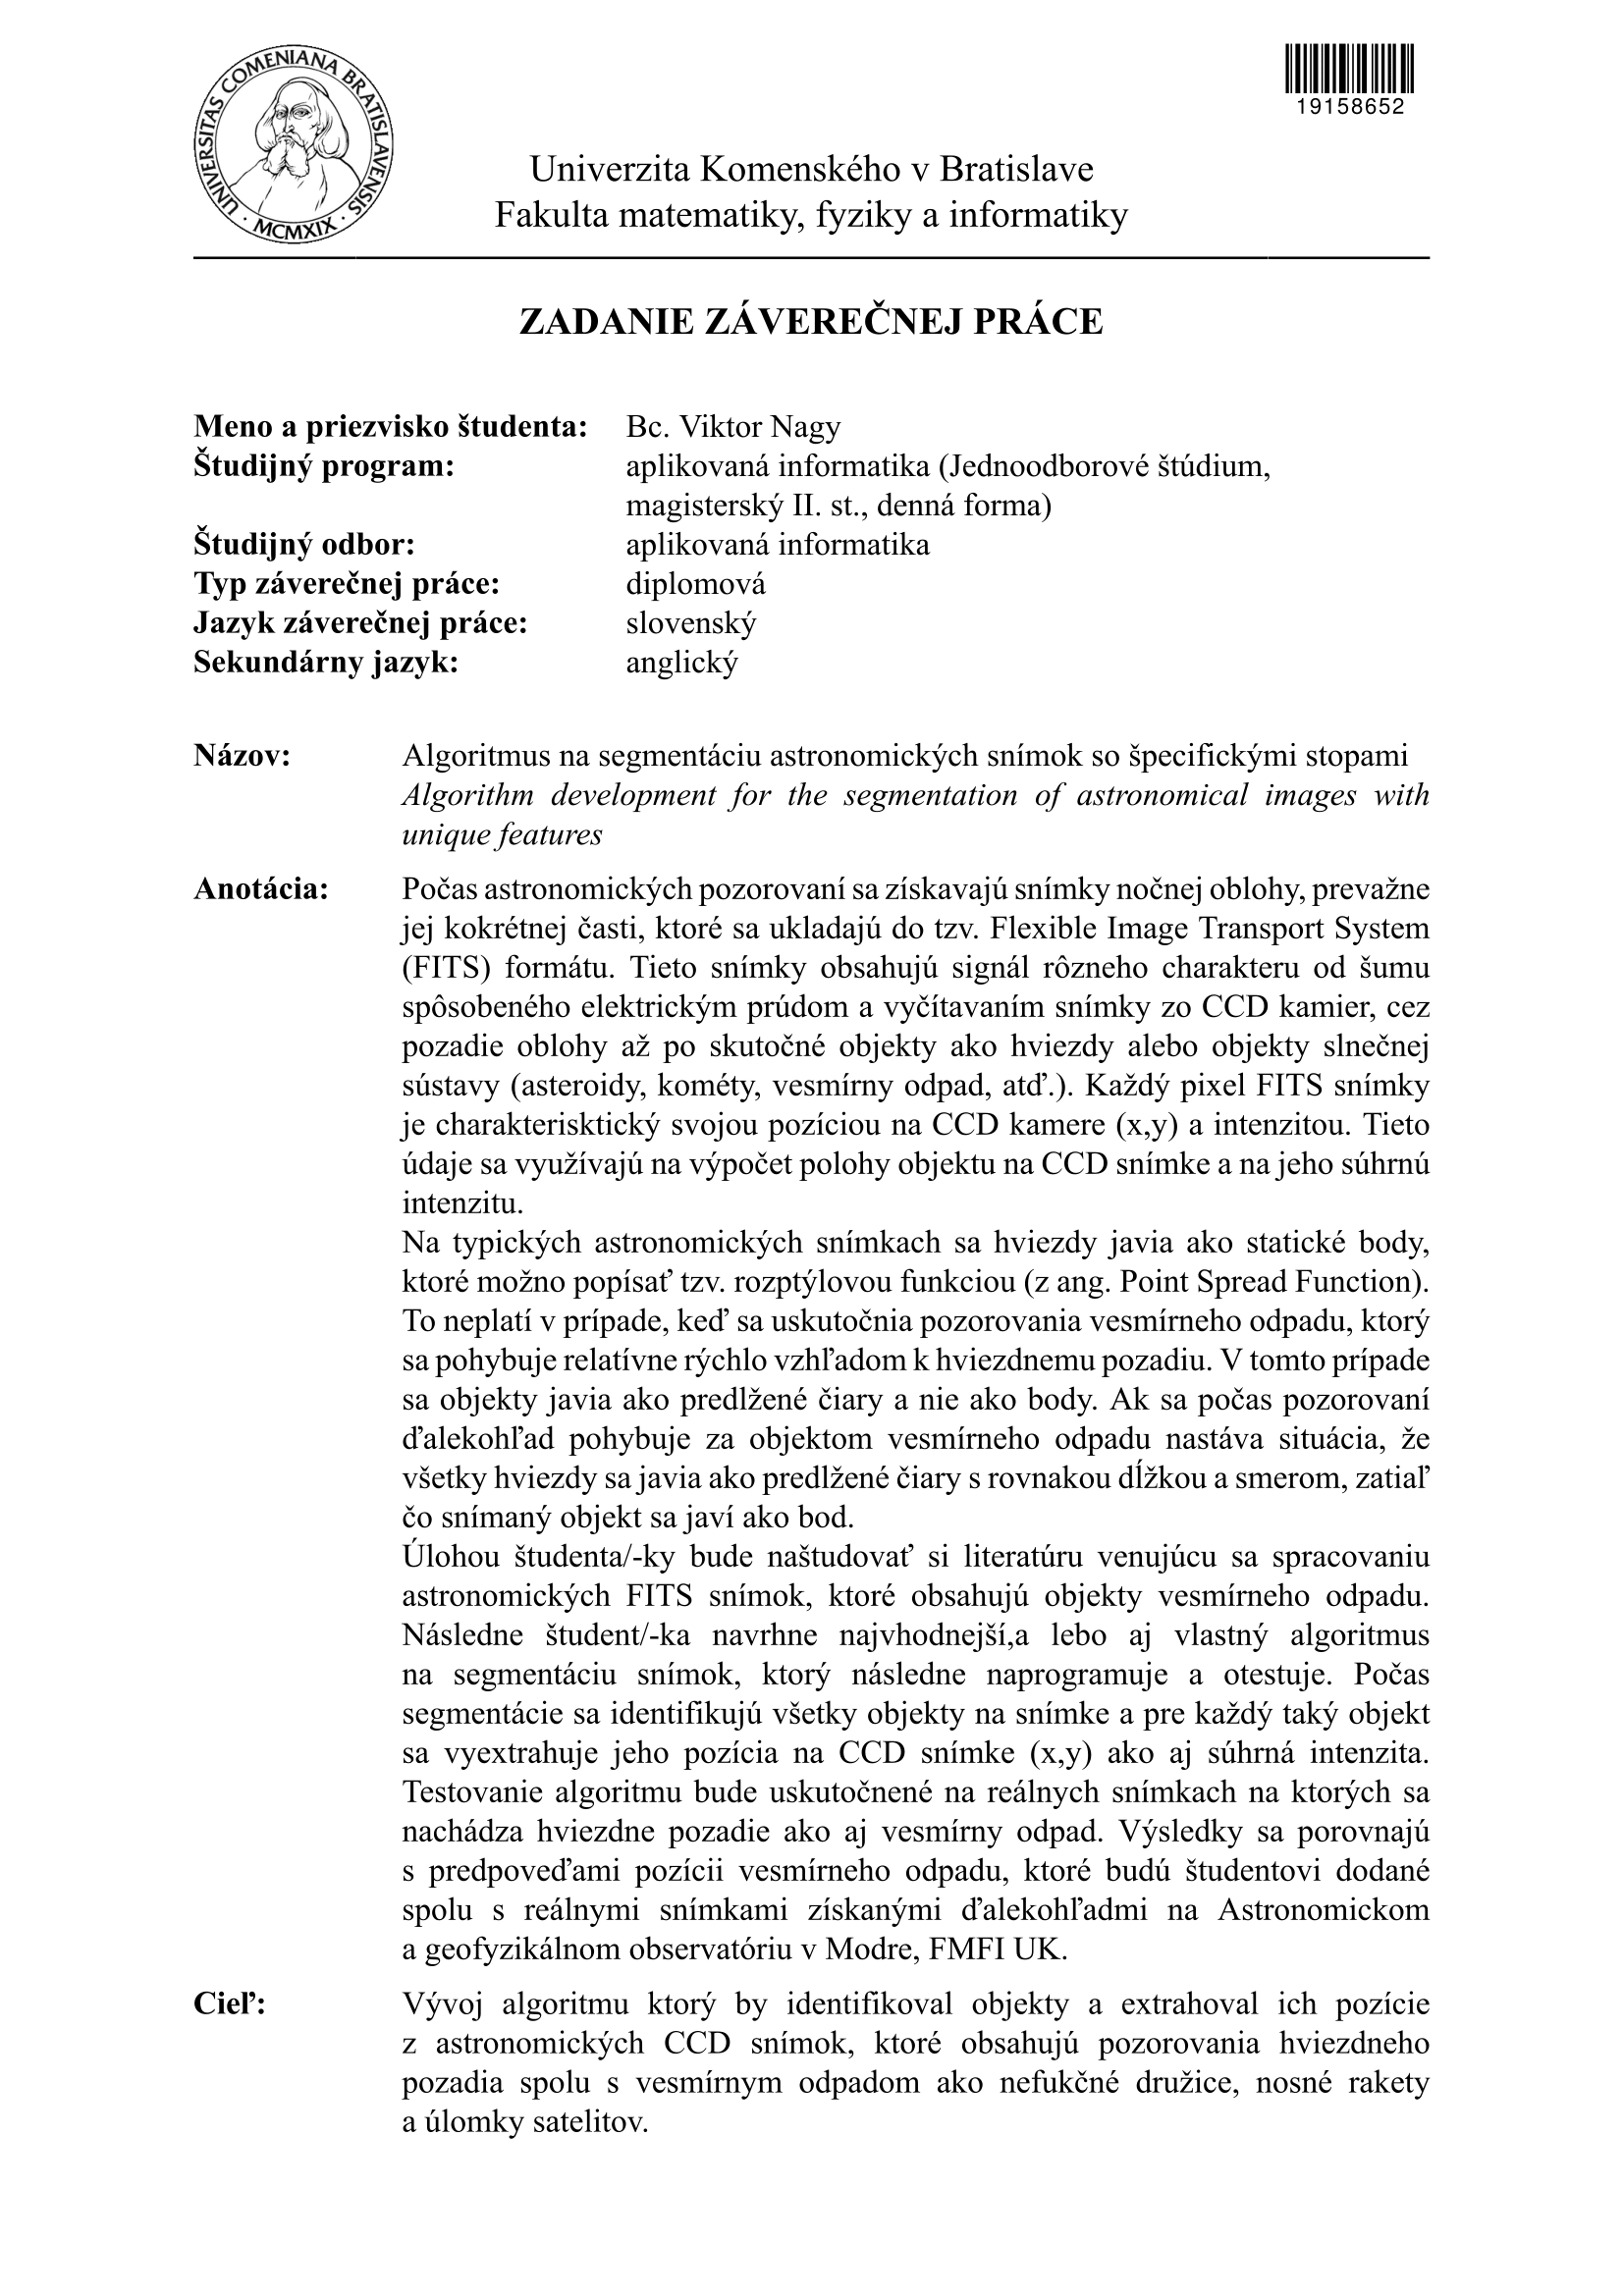
\includegraphics[width=\paperwidth]{zadanie1.png}}
\label{img:zadanie}
\end{center}
\end{figure}

\begin{figure}[H]
\begin{center}
\makebox[\textwidth]{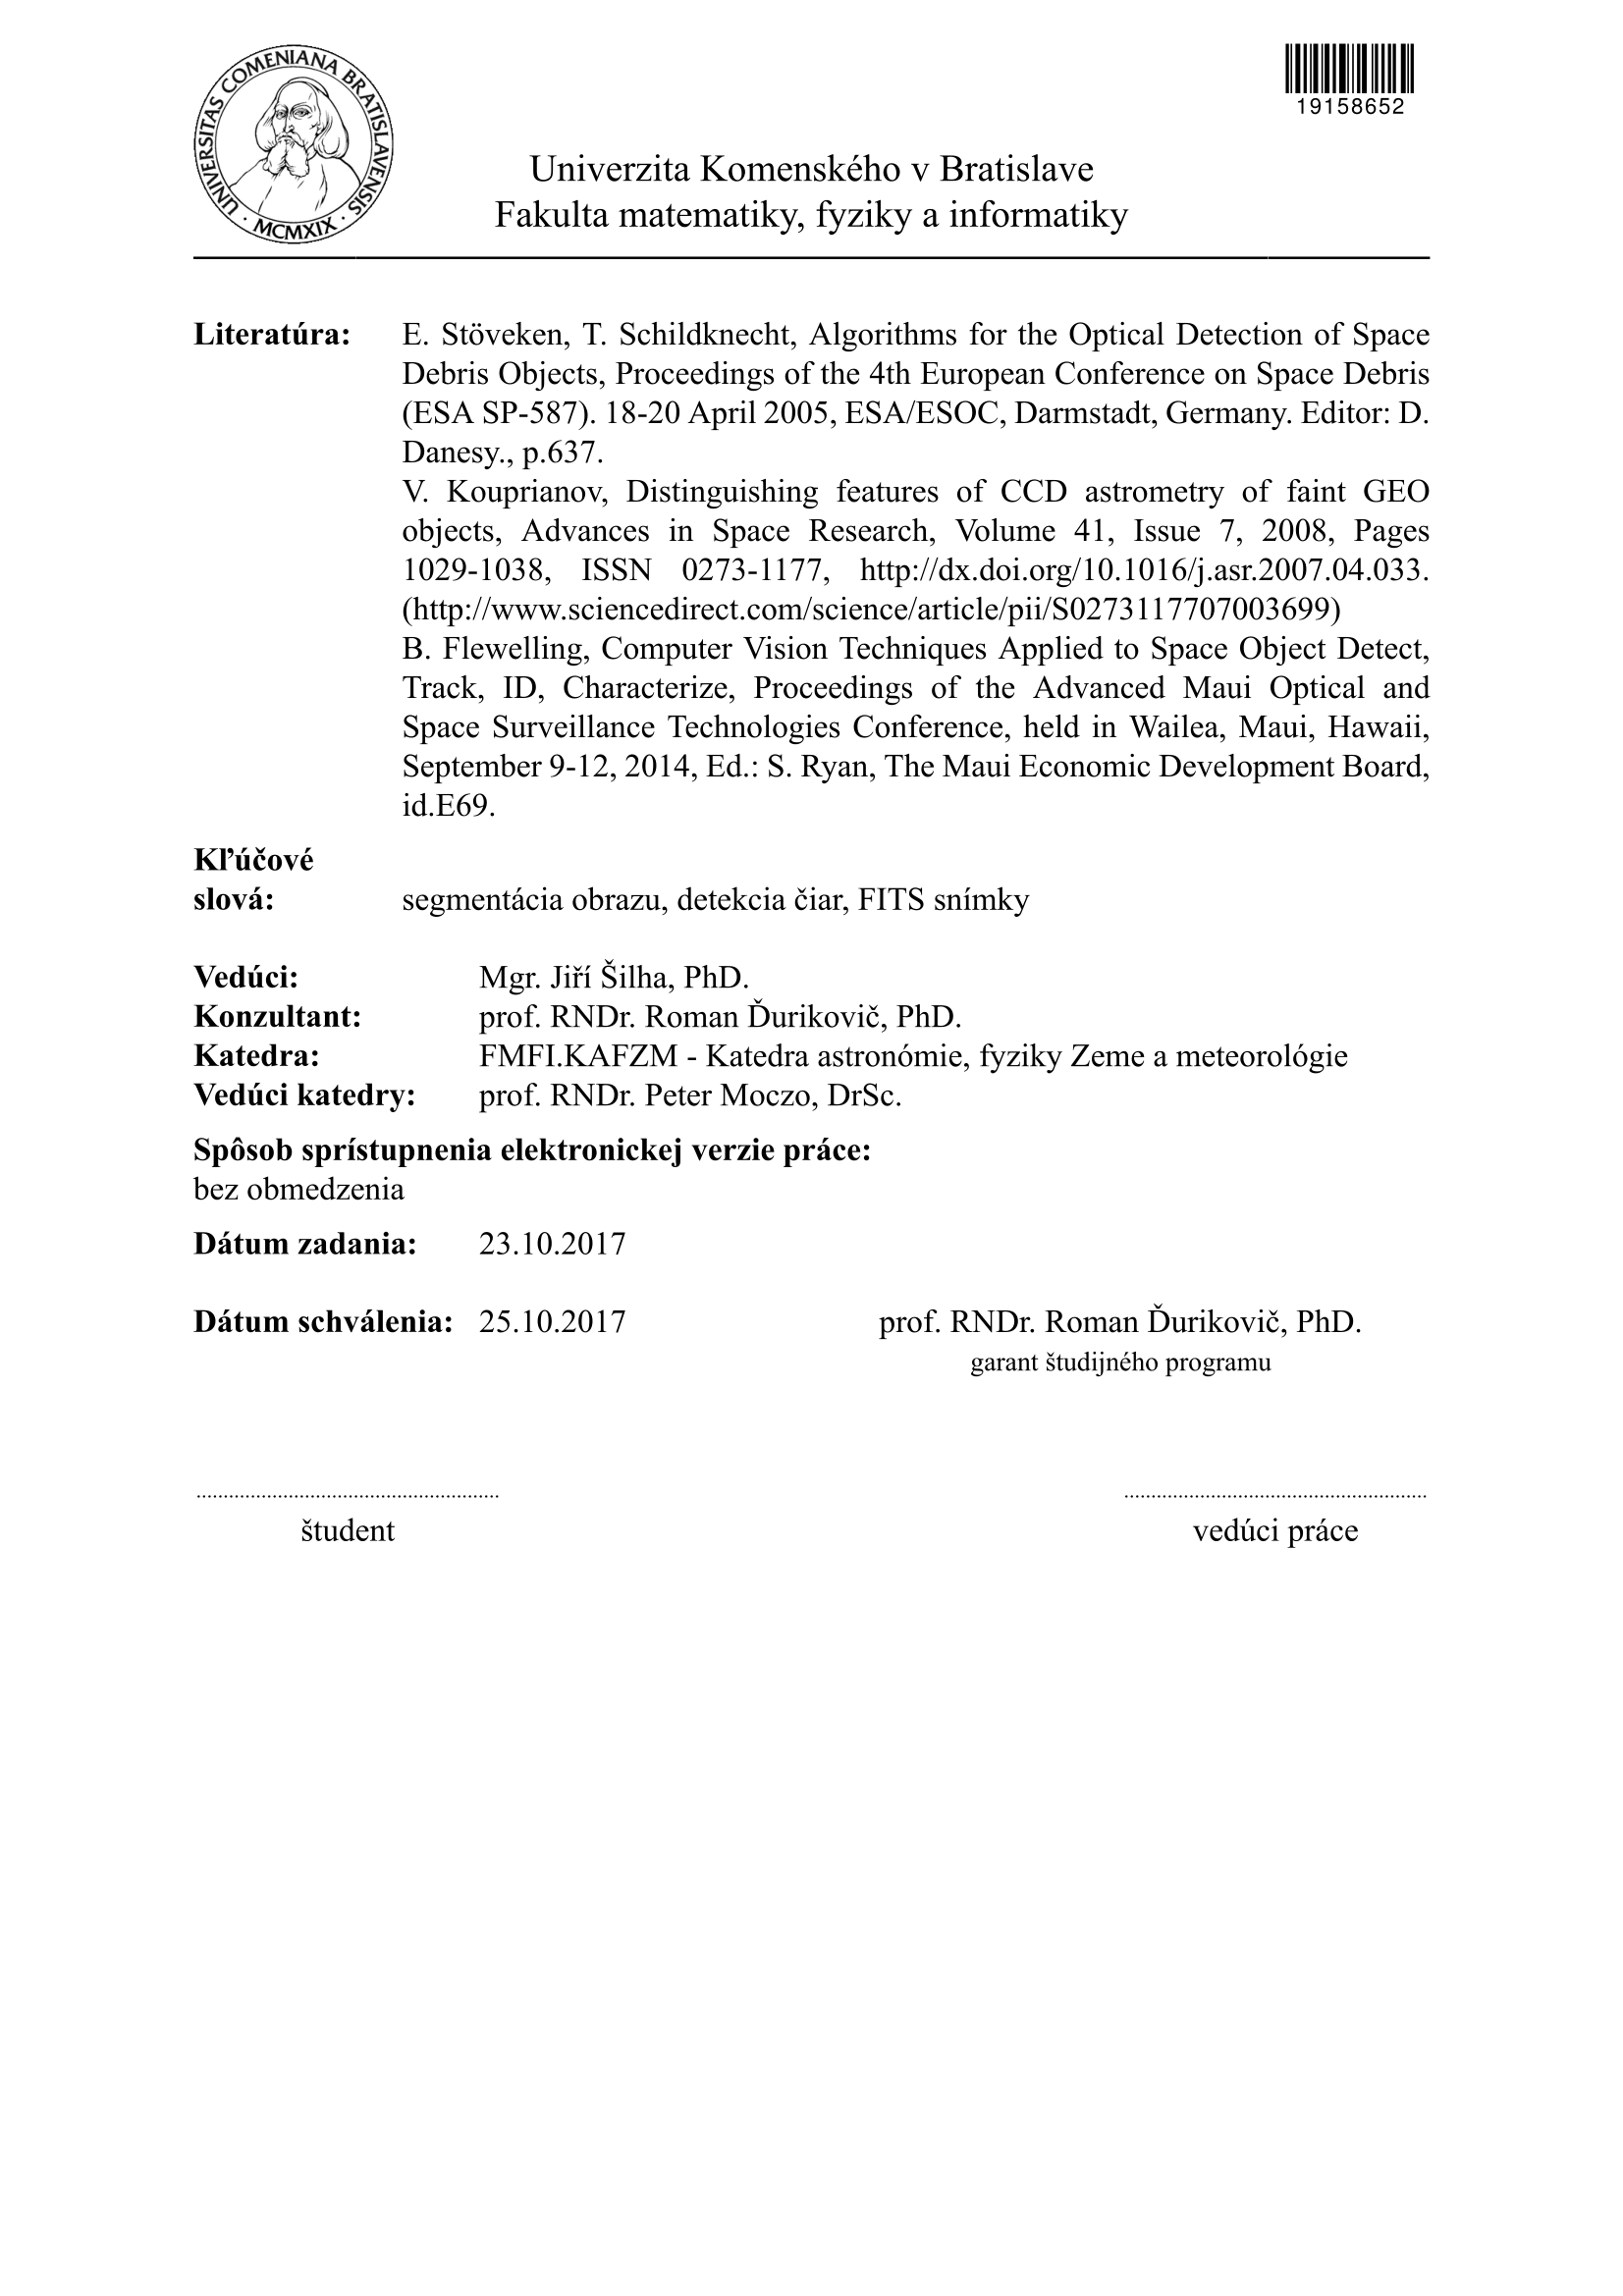
\includegraphics[width=\paperwidth]{zadanie2.png}}
\label{img:zadanie}
\end{center}
\end{figure}


\noindent
\begin{minipage}{0.25\textwidth}~\end{minipage}
\begin{minipage}{0.75\textwidth}
Čestne prehlasujem, že túto diplomovú prácu som vypracoval samostatne len s použitím uvedenej literatúry a za pomoci konzultácií u môjho školiteľa.
\newline \newline
\end{minipage}
\vfill
~ \hfill {\hbox to 6cm{\dotfill}} \\
\mfplacedate \hfill \mfauthor
\vfill\eject 
% koniec prehlasenia

\chapter*{Poďakovanie}\label{chap:thank_you}
\vfill\eject 
% koniec podakovania

\chapter*{Abstrakt}\label{chap:abstract_sk}
Počas astronomických pozorovaní sa získavajú snímky nočnej oblohy, prevažne jej kokrétnej časti, ktoré sa ukladajú do tzv. Flexible Image Transport System (FITS) formátu. Tieto snímky obsahujú signál rôzneho charakteru od šumu spôsobeného elektrickým prúdom a vyčítavaním snímky zo CCD kamier, cez pozadie oblohy až po skutočné objekty ako hviezdy alebo objekty slnečnej sústavy (asteroidy, kométy, vesmírny odpad, atď.). Každý pixel FITS snímky je charakterisktický svojou pozíciou na CCD kamere (x,y) a intenzitou. Tieto údaje sa využívajú na výpočet polohy objektu na CCD snímke a na jeho súhrnú intenzitu.
Na typických astronomických snímkach sa hviezdy javia ako statické body, ktoré možno popísať tzv. rozptýlovou funkciou (z ang. Point Spread Function). To neplatí v prípade, keď sa uskutočnia pozorovania vesmírneho odpadu, ktorý sa pohybuje relatívne rýchlo vzhľadom k hviezdnemu pozadiu. V tomto prípade sa objekty javia ako predlžené čiary a nie ako body. Ak sa počas pozorovaní ďalekohľad pohybuje za objektom vesmírneho odpadu nastáva situácia, že všetky hviezdy sa javia ako predlžené čiary s rovnakou dĺžkou a smerom, zatiaľ čo snímaný objekt sa javí ako bod. 
Úlohou študenta/-ky bude naštudovať si literatúru venujúcu sa spracovaniu astronomických FITS snímok, ktoré obsahujú objekty vesmírneho odpadu. Následne študent/-ka navrhne najvhodnejší,a lebo aj vlastný algoritmus na segmentáciu snímok, ktorý následne naprogramuje a otestuje. Počas segmentácie sa identifikujú všetky objekty na snímke a pre každý taký objekt sa vyextrahuje jeho pozícia na CCD snímke (x,y) ako aj súhrná intenzita. Testovanie algoritmu bude uskutočnené na reálnych snímkach na ktorých sa nachádza hviezdne pozadie ako aj vesmírny odpad. Výsledky sa porovnajú s predpoveďami pozícii vesmírneho odpadu, ktoré budú študentovi dodané spolu s reálnymi snímkami získanými ďalekohľadmi na Astronomickom a geofyzikálnom observatóriu v Modre, FMFI UK.
~\\
Kľúčové slová: debris detection, image processing
\vfill\eject 

\chapter*{Abstract}\label{chap:abstract_en}
During the astronomical observations images are acquired in so-called Flexible Image Transport System (FITS) format. This images contain signal from various sources, starting from electronic noise and readout noise, going trough sky background signal to object images such as stars or asteroids. On an typical astronomical image the stars and asteroids usually appear as point-like objects which can be described by the Point-Spread Function (PSF). This is not the case for the observations of space debris objects such as fragmentation debris, defunct satellites and upper stages. These objects move comparable faster than the stars in the background which leads to FITS images which have present trail-like objects. In case that sidereal tracking is used during the observations, stars are being tracked by the telescope, the space debris object appears as an trail and stars as points. In case that debris tracking is used the debris appears as a point and stars as a trails with the same length and direction on the image. One of the tasks for the possible candidate will be to review the existing algorithms for the image segmentation procedures currently used in the astronomical community for space debris observations. Depending on the review selected will the best algorithm which will be then written by the candidate in a testing environment and then will be tested on the real observations acquired by the optical systems currently present at the Astronomical and geophysical observatory in Modra. Algorithm will have to identify all image objects above defined thershold (Signal-to-Noise Ratio, SNR, to be defined during the work), for each image object extracted will be the position on the CCD frame, as well the total intensity. The algorithm efficiency will be investigated by comparing the results with the ground-truth extracted for the known objects, such as space debris or asteroids which will be delivered to the candidate.


~\\
Keywords: debris detection, image processing
\vfill\eject 
% koniec abstraktov

\tableofcontents

\mainmatter

% treba este prejst dokument ci je kod spravne formatovany
% \input 01intro.tex
% \input 02motivation.tex
% \input 03issues_overview.tex
% \input 04previous_solutions.tex
% \input 05proposal.tex
% \input 06implementation.tex
% \input 07results.tex
% \input 08conclusion.tex

\backmatter

\nocite{*}
\bibliographystyle{alpha}
\bibliography{references}

\listoffigures

\end{document}
